\chapter{Modello a scambio di messaggi}

\section{Caratteristiche del modello}
\begin{figure}[H]
    \centering
    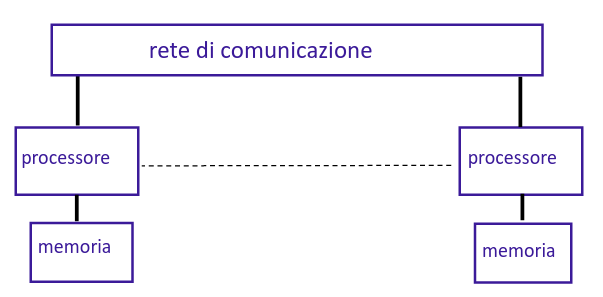
\includegraphics[width=0.6\textwidth]{/home/riccardoob/appunti/sistemi_operativi/images/38.png}
\end{figure}

Ogni processo può accedere \textit{esclusivamente} alle risorse allocate nella \textit{propria memoria locale}, ogni risorsa è quindi accessibile da un solo processo, il \textbf{gestore della risorsa}.

Se una risorsa è necessaria a più processi, ognuno di questi \textbf{processi clienti} deve delegare le operazioni all'unico processo gestore, il quale restituirà gli eventuali risultati.

Ognuno dei processi che necessita di usufruire dei servizi offerti da una risorsa, dovrà \textbf{comunicare} con il gestore, il meccanismo base per permettere questa comunicazione è lo \textbf{scambio di messaggi}.

\section{Canali di comunicazione}
\begin{mdframed}[topline=false,bottomline=false,rightline=false]
Un \textbf{canale} è un collegamento logico mediante il quale due o più processi comunicano.
\end{mdframed}

L'astrazione di canale è realizzata dal nucleo della macchina concorrente, come meccanismo primitivo per lo scambio di informazioni.

Il compito del linguaggio di programmazione è quello di fornire gli strumenti linguistici di alto livello per:
\begin{itemize}
    \item \textit{specificare i canali} di comunicazione
    \item utilizzarli per esprimere le interazioni tra i processi
\end{itemize}

\subsection{Caratteristiche}
I parametri che caratterizzano l'astrazione di canale sono:
\begin{itemize}
    \item \textbf{direzione del flusso di dati} che un canale può trasferire
    \item designazione dei processi \textbf{origine} e \textbf{destinatario} di ogni comunicazione
    \item il \textbf{tipo di sincronizzazione} tra i processi comunicanti
\end{itemize}

\section{Tipi di canale}
Distinguendo la direzione del \textit{flusso di dati}, si denotano due tipi:
\begin{itemize}
    \item canale \textbf{monodirezionale}, consente il flusso di messaggi in una sola direzione
    \item canale \textbf{bidirezionale}, consente di inviare e ricevere messaggi
\end{itemize}
Distinguendo la \textit{designazione dei processi}, si definiscono tre tipi:
\begin{itemize}
    \item \textbf{link}: uno a uno (canale \textbf{simmetrico})
    \item \textbf{port}: molti a uno (canale \textbf{asimmetrico})
    \item \textbf{mailbox}: molti a molti (canale \textbf{asimmetrico}
\end{itemize}

\subsubsection{Link}
\begin{figure}[H]
    \centering
    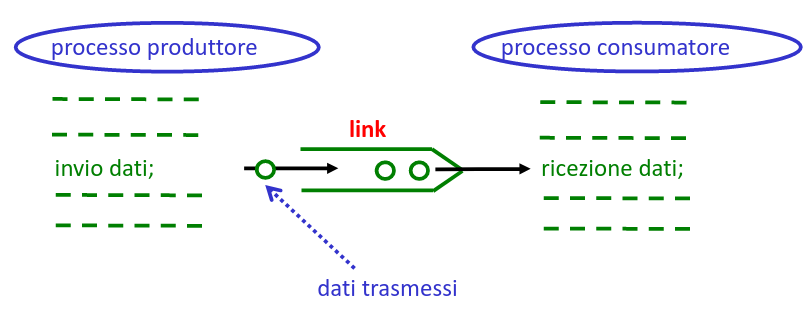
\includegraphics[width=0.6\textwidth]{/home/riccardoob/appunti/sistemi_operativi/images/39.png}
\end{figure}
\subsubsection{Port}
\begin{figure}[H]
    \centering
    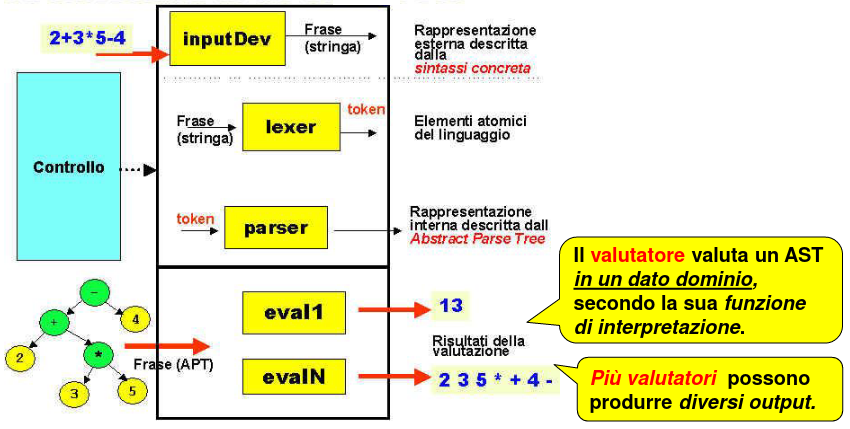
\includegraphics[width=0.6\textwidth]{/home/riccardoob/appunti/sistemi_operativi/images/40.png}
\end{figure}

Distinguendo la modalità di \textbf{sincronizzazione} tra i processi comunicanti, si individuano tre tipi:
\begin{itemize}
    \item comunicazione \textbf{asincronia}
    \item comunicazione \textbf{sincrona}
    \item comunicazione con \textbf{sincronizzazione estesa}
\end{itemize}

\subsection{Comunicazione asincrona}
Il processo \textit{continua la sua esecuzione} immediatamente dopo l'invio del messaggio.

Il messaggio viene ricevuto in un istante successivo all'invio, le informazioni contenute nel messaggio \textit{non possono essere attribuite allo stato attuale} del mittente.

L'invio di un messaggio \textit{non è un punto di sincronizzazione} tra mittente e destinatario.

\subsubsection{Proprietà}
\begin{itemize}
    \item \textbf{carenza espressiva}
    \item \textbf{assenza di vincoli di sincronizzazione} favorisce il grado di concorrenza
    \item sarebbe necessario un buffer di \textit{capacità illimitata}
\end{itemize}

Ogni implementazione prevede un limite alla capacità del buffer, in caso di \textit{buffer pieno}, è necessario sospendere il processo che invia il messaggio.

\subsection{Comunicazione sincrona - randez-vous semplice}
Il primo dei due processi comunicanti che esegue l'invio o la ricezione, si \textbf{sospende}, in attesa che l'altro esegua l'operazione corrispondente.

L'invio di un messaggio è un \textit{punto di sincronizzazione}, ogni messaggio può essere attribuito allo stato attuale del mittente.

Non è necessaria l'introduzione di un buffer, in quanto un messaggio può essere inviato solo se ildestinatario è pronto a riceverlo.

\subsubsection{Realizzazione canale sincrono tramite comunicazioni asincrone}
\begin{figure}[H]
    \centering
    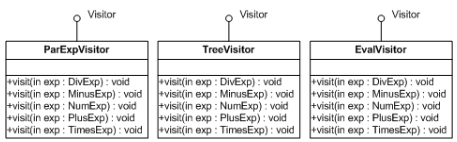
\includegraphics[width=0.6\textwidth]{/home/riccardoob/appunti/sistemi_operativi/images/41.png}
\end{figure}

\subsection{Comunicazione con sincronizzazione estesa - randez-vous esteso}
Si assume che ogni messaggio inviato rappresenta una richiesta al destinatario di una esecuzione di \textit{una certa azione}.

Il mittente rimane in attesa fino a che il ricevente non ha terminato di svolgere l'azione richiesta:
\begin{itemize}
    \item vero e proprio modello \textbf{cliente-servitore}
    \item analogia semantica con \textbf{chiamata di procedura}
    \item riduzione del parallelismo
\end{itemize}

\begin{figure}[H]
    \centering
    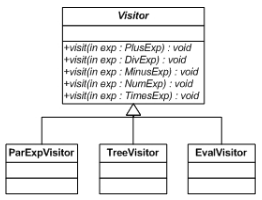
\includegraphics[width=0.6\textwidth]{/home/riccardoob/appunti/sistemi_operativi/images/42.png}
\end{figure}

\section{Costrutti linguistici e primitive per esprimere la comunicazione}


\subsubsection{Definizione del canale}

\begin{minted}[bgcolor=lightgray,framesep=2mm,baselinestretch=1.2,fontsize=\footnotesize,escapeinside=||,mathescape=true]{go}
port <tipo> <identificatore>;
\end{minted}

\texttt{port} viene dichiarato locale a un processo, ed è visibile ai processi mittenti tramite dot notation.
\begin{minted}[bgcolor=lightgray,framesep=2mm,baselinestretch=1.2,fontsize=\footnotesize,escapeinside=||,mathescape=true]{go}
<nome processo>.<identificatore canale>
\end{minted}

\subsection{Primitive di comunicazione}

\subsubsection{Send}

\texttt{send} esprime l'invio di un messaggio
\begin{minted}[bgcolor=lightgray,framesep=2mm,baselinestretch=1.2,fontsize=\footnotesize,escapeinside=||,mathescape=true]{go}
send(<valore>) to <porta>;
\end{minted}

\texttt{<porta>} individua il canale a cui inviare il messaggio, \texttt{<valore>} è il contenuto del messaggio.

La semantica dipende dal tipo di canale: sincrono o asincrono.

\subsubsection{Receive}
\begin{minted}[bgcolor=lightgray,framesep=2mm,baselinestretch=1.2,fontsize=\footnotesize,escapeinside=||,mathescape=true]{go}
P = receive(<variabile>) from <porta>;
\end{minted}

\begin{itemize}
    \item \texttt{<porta>} identifica il canale, locale al ricevente, dal quale ricevere il messaggio
    \item \texttt{<variabile>} è l'identificatore della variabile a cui assegnare il valore del messaggio ricevuto
\end{itemize}

Di default la semantica è \textbf{bloccante} in caso di buffer vuoto, con attesa di un messaggio, alcuni linguaggi offrono anche una semantica non bloccante.

\subsection{Receive bloccante e modello C/S}

Il \textbf{server} è un processo dedicato a servire le richieste di altri processi (clienti), ognuna rappresentata da un diverso messaggio.

Il server può offrire diversi servizi, ognuno attivato dalla ricezione di un messaggio su un particolare canale, quindi il server gestisce tanti \textbf{canali di ingresso} quanti sono i servizi che offre

Nasce il problema della \texttt{receive} bloccante, si può infatti ottenere un server bloccato su una \texttt{receive} su un canale vuoto, mentre ci sono altri canali non vuoti in attesa di essere serviti.

É necessario implementare una receive con semantica non bloccante: si verifica lo stato del canale e si restituisce un messaggio se presente, altrimenti una segnalazione di canale vuoto.

Sorge tuttavia il problema dell'\textbf{attesa attiva} nel caso in cui tutti i canali siano vuoti.

Il meccanismo di ricezione ideale:
\begin{itemize}
    \item permette al processo server di verificare \textbf{contemporaneamente} la disponibilità di messaggi su più canali
    \item abilita la ricezione di un messaggio da \textit{qualunque canale contenente messaggi}
    \item quando tutti i canali sono vuoti, blocca il processo in attesa che arrivi un messaggio (su qualunque canale)
\end{itemize}

\subsection{Comando con guardia}
\begin{minted}[bgcolor=lightgray,framesep=2mm,baselinestretch=1.2,fontsize=\footnotesize,escapeinside=||,mathescape=true]{go}
<guardia> -> <istruzione>;
\end{minted}
dove guardia è costituito dalla coppia
\begin{minted}[bgcolor=lightgray,framesep=2mm,baselinestretch=1.2,fontsize=\footnotesize,escapeinside=||,mathescape=true]{go}
(<espressione booleana>; <receive>)
\end{minted}

L'espressione booleana viene detta \textbf{guardia logica}, la receive ha semantica bloccante e viene detta \textbf{guardia d'ingresso}.

La valutazione di una guardia ha tre possibili risultati:
\begin{itemize}
    \item \textbf{guardia fallita}: espressione booleana è \texttt{false}
    \item \textbf{guardia ritardata}: espressione booleana è \texttt{true} ma non ci sono messaggi
    \item \textbf{guardia valida}: espressione booleana \texttt{true} ed è presente almeno un messaggio
\end{itemize}

In caso di
\begin{itemize}
    \item \textbf{guardia fallita}, l'istruzione non viene eseguita
    \item \textbf{guardia ritardata}, il processo viene sospeso e riattivato una volta arrivato un messaggio sulla guardia d'ingresso, si esegue la receive e successivamente l'istruzione
    \item \textbf{guardia valida}, il processo esegue la receive e successivamente l'istruzione
\end{itemize}

\subsection{Comando con guardia alternativo}
\begin{minted}[bgcolor=lightgray,framesep=2mm,baselinestretch=1.2,fontsize=\footnotesize,escapeinside=||,mathescape=true]{go}
select
{
    [] <guardia_1> -> <istruzione_1>;
    [] <guardia_2> -> <istruzione_2>;
    ...
    [] <guardia_n> -> <istruzione_n>;
}
\end{minted}

Il comando di guardia alternativo racchiude un numero arbitrario di comandi con guardia semplici.

La semantica si basa sulla valutazione delle guardie di tutti i rami, tre casi:
\begin{itemize}
    \item \textbf{una o più guardie valide}: eseguito in maniera \textbf{non deterministica} uno dei rami
    \item \textbf{tutte le guardie non fallite sono ritardate}: il processo attende un messaggio che abiliti l'esecuzione di una guardia ritardata
    \item \textbf{tutte le guardie sono fallite}: il comando termina
\end{itemize}

\subsection{Comando con guardia ripetitivo}
\begin{minted}[bgcolor=lightgray,framesep=2mm,baselinestretch=1.2,fontsize=\footnotesize,escapeinside=||,mathescape=true]{go}
do
{
    [] <guardia_1> -> <istruzione_1>;
    [] <guardia_2> -> <istruzione_2>;
    ...
    [] <guardia_n> -> <istruzione_n>;
}
\end{minted}

Stessa semantica del comando con guardia alternativo ma viene iterato una volta terminato il comando.

\subsubsection{Esempio processo servitore}
\begin{minted}[bgcolor=lightgray,framesep=2mm,baselinestretch=1.2,fontsize=\footnotesize,escapeinside=||,mathescape=true]{go}
processo server {
    port int canale1;
    port real canale2;
    Tipo_di_R R;
    int x;
    real y;
    do {
        [] (cond1); receive (x) from canale1; ->
        {
            R.S1;
            <eventuale restituzione al cliente>;
        }
        [] (cond2); receive (x) from canale2; ->
        {
            R.S2;
            <eventuale restituzione al cliente>;
        }
    }
}
\end{minted}

\section{Primitive di comunicazione asincrone}

Nel modello a scambio di messaggi, lo strumento di comunicazione di più basso livello è la \textbf{send asincrona}, che abilita l'accesso a risorse "condivise" tramite processi servitori.

\subsection{Problemi di sincronizzazione}
Si prendono in considerazione alcuni tipici problemi di interazone nel modello a scambio di messaggi con send asincrona per realizzare un gestore di risorse dei tipi:
\begin{itemize}
    \item una sola operazione
    \item più operazioni mutuamente esclusive
    \item più operazioni con condizioni di sincronizzazione
\end{itemize}

Si individuano ora schemi di soluzioni alle diverse problematiche.

\subsubsection{Esempio - risorsa condivisa con una sola operazione}
La risorsa viene gestita da un processo server, che offre un unico servizio senza condizioni di sincronizzazione:
\begin{multicols}{2}
    \begin{minted}[bgcolor=lightgray,framesep=2mm,baselinestretch=1.2,fontsize=\footnotesize,escapeinside=||,mathescape=true]{go}
process cliente {
    port tipo_out risposta;
    tipo_in a;
    tipo_out b;
    process p;
    ...
    send(a) to server.input;
    p = receive(b) from risposta;
    ...
}
    \end{minted}
    \columnbreak
    \begin{minted}[bgcolor=lightgray,framesep=2mm,baselinestretch=1.2,fontsize=\footnotesize,escapeinside=||,mathescape=true]{go}
tipo_out fun(tipo_in x);
process server {
    port tipo_in input;
    tipo_var var;
    process p;
    tipo_in x;
    tipo_out y;
    <inizializzazione>;
    while (true) {
        p = receive (x) from input;
        y = fun(x);
        send (y) to p.risposta;
    }
}
    \end{minted}
\end{multicols}

\subsubsection{Esempio - risorsa condivisa con più operazioni}
La risorsa è gestita da un processo server che offre due servizi senza condizioni di sincronizzazione.

Soluzione senza comandi guardia

\begin{minted}[bgcolor=lightgray,framesep=2mm,baselinestretch=1.2,fontsize=\footnotesize,escapeinside=||,mathescape=true]{go}
typedef struct {
    enum (fun1, fun2) servizio;
    union {
        tipo_in1 x1; //parametri fun1
        tipo_in2 x2; //parametri fun2
    } parametri
} in_mess;
\end{minted}

\begin{minted}[bgcolor=lightgray,framesep=2mm,baselinestretch=1.2,fontsize=\footnotesize,escapeinside=||,mathescape=true]{go}
tipo_out1 fun1 (tipo_in1 x1);
tipo_out2 fun2 tipo_in2 x2);

process server {
    port in_mess input;
    tipo_var var;
    process p;
    in_mes richiesta;
    tipo_out1 y1;
    tipo_out2 y2;

    while (true) {
        p = receive(richiesta) from input;
        switch (richiesta.servizio) {
            case fun1: {
                y1 = fun1(richiesta.parametri.x1);
                send (y1) to p.risposta1;
                break;
            }
            case fun2: { 
                y2 = fun2(richiesta.parametri.x2);
                send (y2) to p.risposta2;
                break;
            }
        }
    }
}

\end{minted}

\begin{minted}[bgcolor=lightgray,framesep=2mm,baselinestretch=1.2,fontsize=\footnotesize,escapeinside=||,mathescape=true]{go}
process cliente {
    port tipo_out1 risposta1;
    port tipo_out2 risposta2;
    tipo_in1 a1;
    tipo_in2 a2;
    in_mes M;
    tipo_out1 b1;
    tipo_out2 b2;
    process p;
    <inizializzazione M, in base al servizio scelto>;
    if (<servizio1>) then {
        send(M) to server.input;
        p = receive (b1) from risposta1;
    }
    else {
        send(M) to server.input;
        p = receive (b2) from risposta2;
    }
    ...
}
\end{minted}

Soluzione con comandi guardia, un canale per ogni servizio.

\begin{minted}[bgcolor=lightgray,framesep=2mm,baselinestretch=1.2,fontsize=\footnotesize,escapeinside=||,mathescape=true]{go}
tipo_out1 fun1(tipo_in1 x1);
tipo_out2 fun2(tipo_in2 x2);
process server {
    port tipo_in1 input1; //canale per le richieste relative a fun1
    port tipo_in2 input2; //canale per le richieste relative a fun2
    tipo_var var;
    process p;
    tipo_in1 x1;
    tipo_in2 x2;
    tipo_out1 y1;
    tipo_out2 y2;
    <eventuale inizializzazione>;
    do {
        [] p = receive (x1) from input1; ->
            y1=fun1(x1);
            send (y1) to p.risposta1;

        [] p = receive (x2) from input2; ->
            y2=fun2(x2);
            send (y2) to p.risposta2;
    }
}
\end{minted}

\begin{minted}[bgcolor=lightgray,framesep=2mm,baselinestretch=1.2,fontsize=\footnotesize,escapeinside=||,mathescape=true]{go}
process cliente {
    port tipo_out1 risposta1;
    port tipo_out1 risposta1;
    tipo_in1 a1;
    tipo_in2 a2;
    tipo_out1 b1;
    tipo_out2 b2;
    process p;
    <inizializzazione a1 o a2>
    if (<servizio1>) then {
        send(a1)to server.input1;
        p=receive(b1)from risposta1;
    }
    else {
        send(a2)to server.input2;
        p=receive(b2)from risposta2;
    }
    ...
}
\end{minted}


GUARDA ESEMPI 50-106
























